\documentclass{article}
\usepackage[margin=1in]{geometry}
\usepackage{graphicx}
\usepackage{hyperref}
\title{\vspace{-2.0cm}ViReport v0.0.1}
\author{Niema Moshiri}
\date{2020-03-16}
\begin{document}
\maketitle

\section{Input Dataset}
The analysis was conducted on a dataset containing 571 sequences.
The average sequence length was 29799.611,
with a standard deviation of 293.817.
The earliest sample date was 2019-12-01,
the median sample date was 2020-02-25,
and the most recent sample date was 2020-03-11.


\begin{figure}[h]
\centering
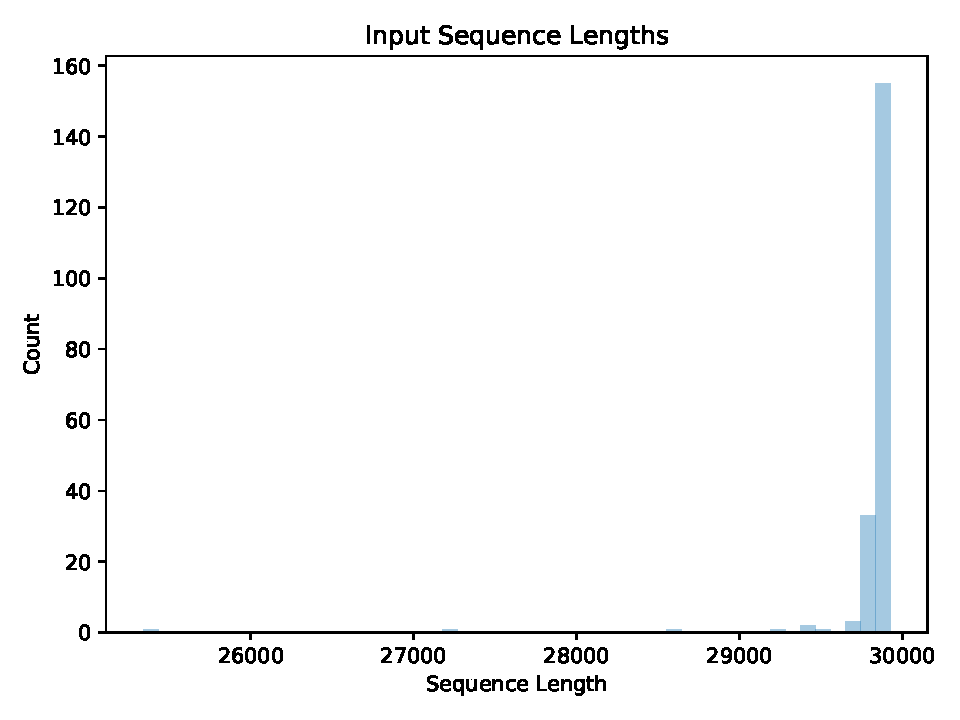
\includegraphics[width=0.75\textwidth,keepaspectratio]{./figs/input_sequence_lengths.pdf}
\caption{Distribution of input sequence lengths}
\end{figure}



\begin{figure}[h]
\centering
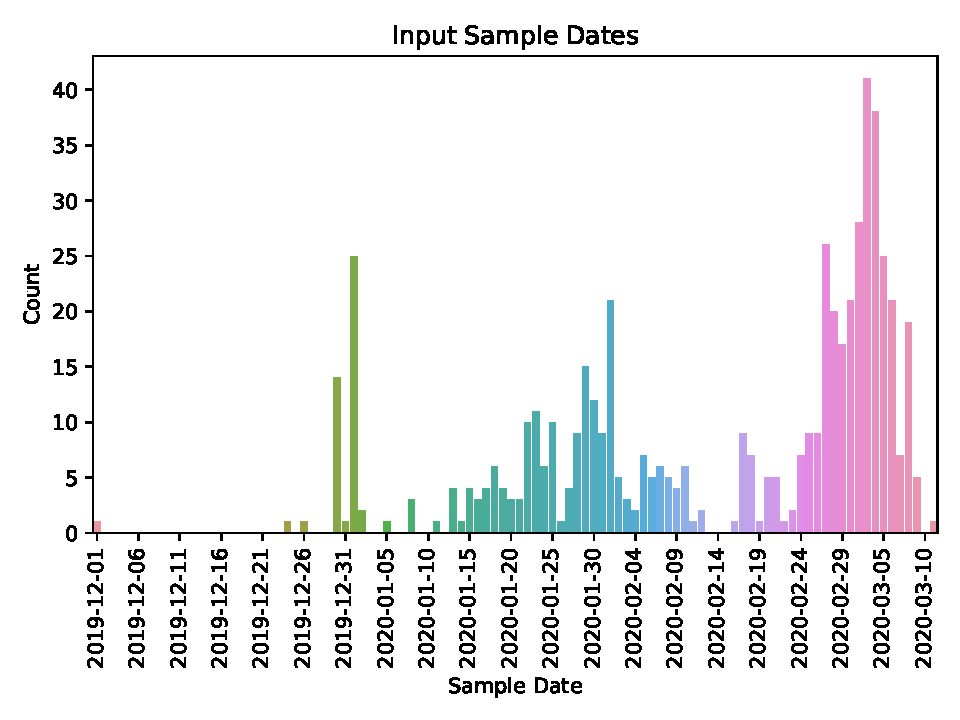
\includegraphics[width=0.75\textwidth,keepaspectratio]{./figs/input_sample_dates.pdf}
\caption{Distribution of input sample dates}
\end{figure}

\section{Preprocessed Dataset}
The input dataset was preprocessed such that sequences were given safe names: non-letters/digits in sequence IDs were converted to underscores.
After preprocessing, the dataset contained 571 sequences.
The average sequence length was 29799.611,
with a standard deviation of 293.817.
The earliest sample date was 2019-12-01,
the median sample date was 2020-02-25,
and the most recent sample date was 2020-03-11.


\begin{figure}[h]
\centering
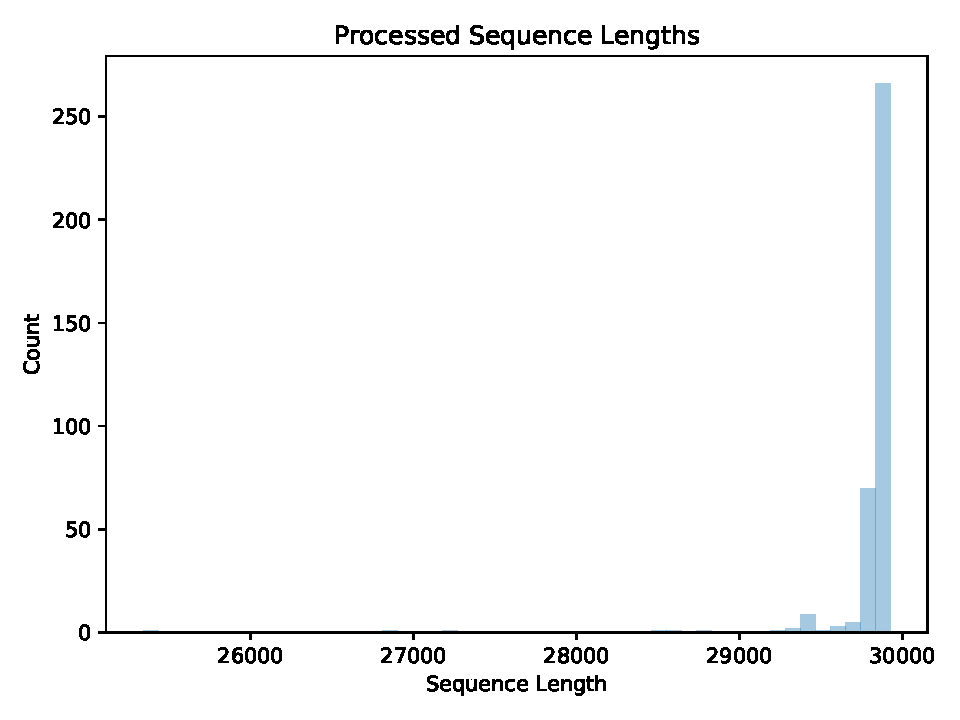
\includegraphics[width=0.75\textwidth,keepaspectratio]{./figs/processed_sequence_lengths.pdf}
\caption{Distribution of preprocessed sequence lengths}
\end{figure}



\begin{figure}[h]
\centering
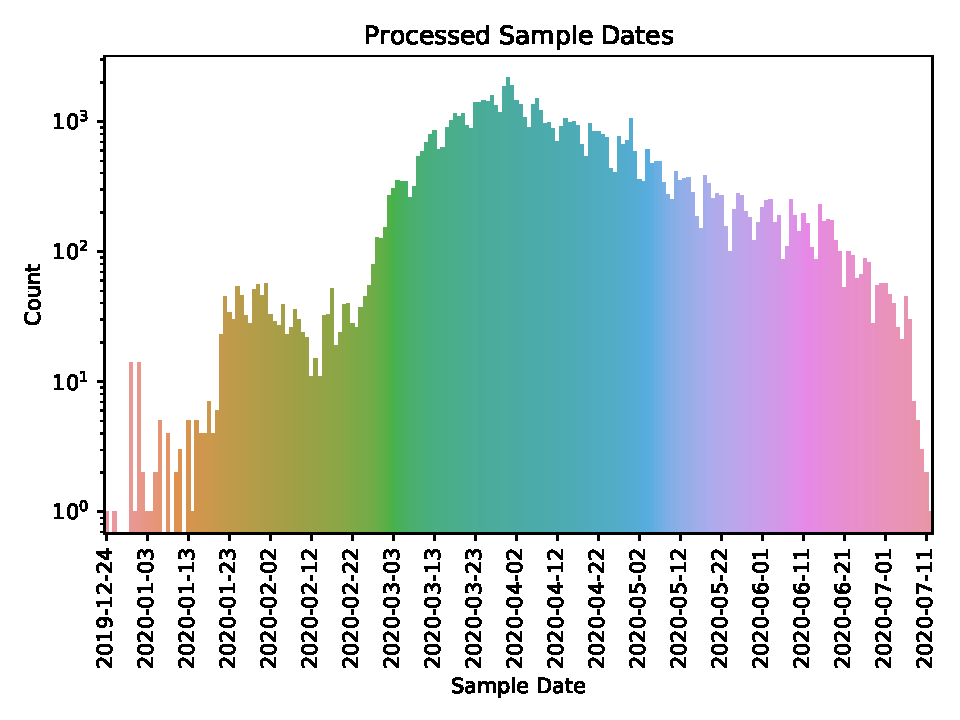
\includegraphics[width=0.75\textwidth,keepaspectratio]{./figs/processed_sample_dates.pdf}
\caption{Distribution of preprocessed sample dates}
\end{figure}

\section{Multiple Sequence Alignment}
Multiple sequence alignment was performed using MAFFT (Katoh \& Standley, 2013) in automatic mode.
There were 30042 positions (6791 invariant) and 512 unique sequences in the multiple sequence alignment.
Pairwise distances were computed from the multiple sequence alignment using the tn93 tool of HIV-TRACE (Pond et al., 2018).
The average pairwise sequence distance was 0.000286,
with a standard deviation of 0.000204.


\begin{figure}[h]
\centering
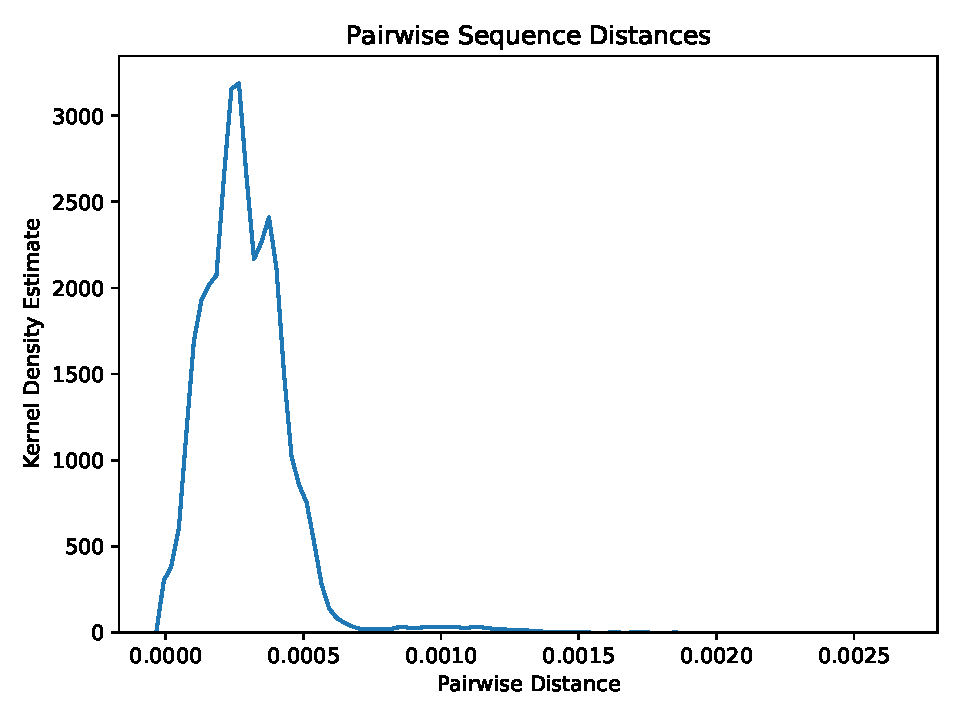
\includegraphics[width=0.75\textwidth,keepaspectratio]{./figs/pairwise_distances_sequences.pdf}
\caption{Distribution of pairwise sequence distances}
\end{figure}

Across the positions of the multiple sequence alignment that had non-zero Shannon entropy,
the minimum Shannon entropy was 0.0189,
the maximum Shannon entropy was 2,
and the average Shannon entropy was 0.062,
with a standard deviation of 0.103.


\begin{figure}[h]
\centering
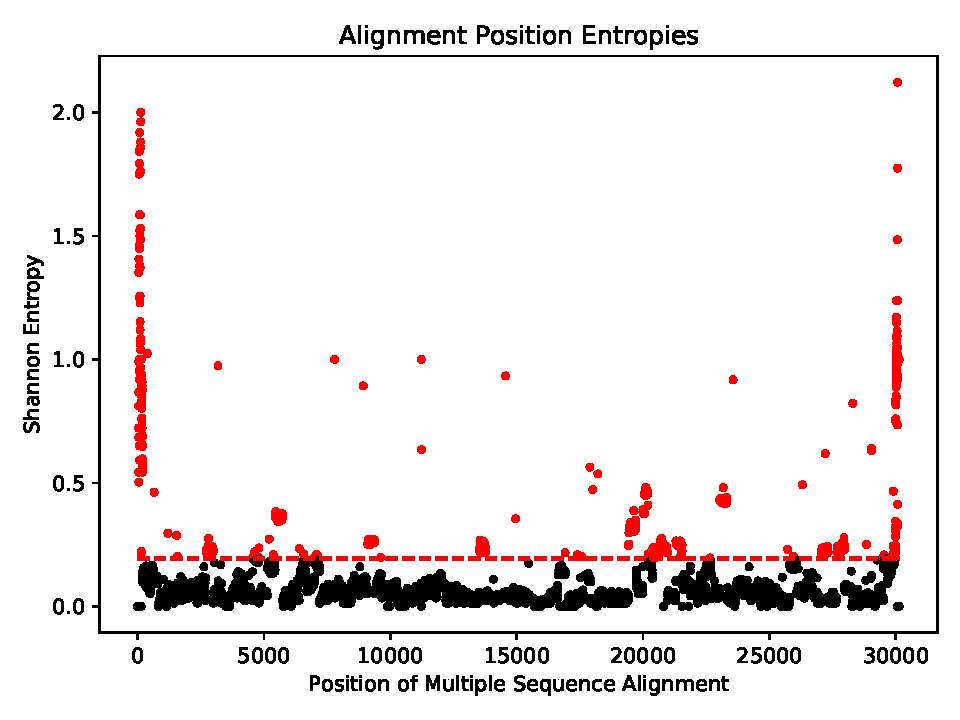
\includegraphics[width=0.75\textwidth,keepaspectratio]{./figs/alignment_entropies.pdf}
\caption{Shannon entropy across the positions of the multiple sequence alignment}
\end{figure}

\section{Phylogenetic Inference}
A maximum-likelihood phylogeny was inferred under the General Time-Reversible (GTR) model (Tavare, 1986) using FastTree 2 (Price et al., 2010) using a Gamma20-based likelihood.
The inferred phylogeny was MinVar-rooted using FastRoot (Mai et al., 2017).
Pairwise distances were computed from the phylogeny using TreeSwift (Moshiri, 2020).
The maximum pairwise phylogenetic distance (i.e., tree diameter) was 0.00479,
and the average pairwise phylogenetic distance was 0.000521,
with a standard deviation of 0.000372.


\begin{figure}[h]
\centering

\includegraphics[width=1\textwidth,height=1\textheight,keepaspectratio]{./figs/tree_mutations.pdf}
\caption{Rooted phylogenetic tree in unit of expected per-site mutations}
\end{figure}



\begin{figure}[h]
\centering
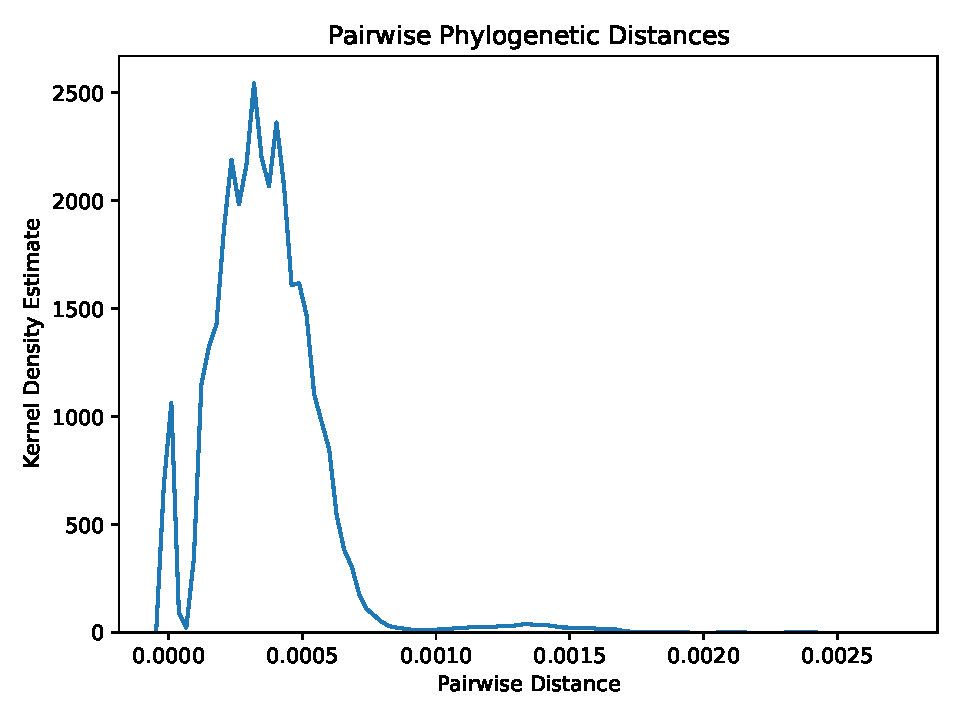
\includegraphics[width=0.75\textwidth,keepaspectratio]{./figs/pairwise_distances_tree.pdf}
\caption{Distribution of pairwise phylogenetic distances}
\end{figure}

\section{Phylogenetic Dating}
The rooted phylogeny was dated using treedater (Volz \& Frost, 2017).
The height of the dated tree was 112.473 days,
so given that the most recent sample was collected on 2020-03-11,
the estimated time of the most recent common ancestor (tMRCA) was 2019-11-19.


\begin{figure}[h]
\centering
\includegraphics[width=1\textwidth,height=1\textheight,keepaspectratio]{./figs/tree_time.pdf}
\caption{Dated phylogenetic tree in unit of years}
\end{figure}

\section{Ancestral Sequence Reconstruction}
Ancestral sequence reconstruction was performed using TreeTime (Sagulenko et al., 2018).
\section{Transmission Clustering}
Transmission clustering was performed using TreeN93 (Moshiri, 2018) using pairwise phylogenetic distances.
The total number of singletons (i.e., non-clustered individuals) was 90,
and the total number of clusters (excluding singletons) was 24.
The average cluster size (excluding singletons) was 19.583,
with a standard deviation of 45.409,
and the maximum and minimum cluster sizes were 215 and 2, respectively.


\begin{figure}[h]
\centering
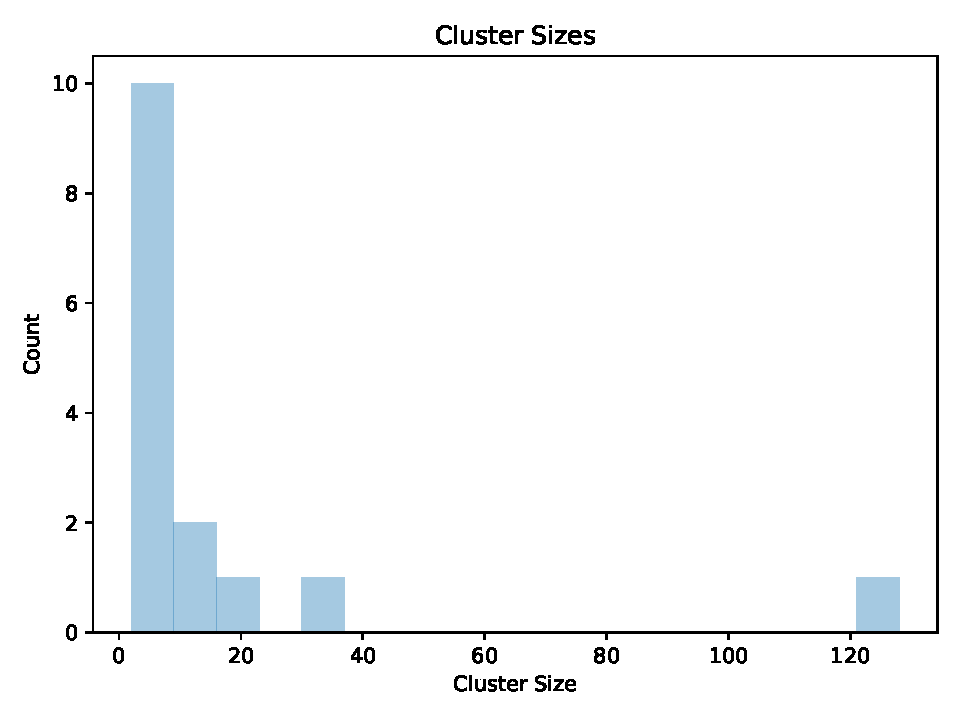
\includegraphics[width=0.75\textwidth,keepaspectratio]{./figs/cluster_sizes.pdf}
\caption{Distribution of cluster sizes (excluding singletons)}
\end{figure}

\section{Citations}
\begin{itemize}
\item Katoh K., Standley D.M. (2013). "MAFFT Multiple Sequence Alignment Software Version 7: Improvements in Performance and Usability". Molecular Biology and Evolution. 30(4), 772-780.\item Le S.Q., Gascuel O. (2008). "An Improved General Amino Acid Replacement Matrix". Molecular Biology and Evolution. 25(7), 1307-1320.\item Mai U., Sayyari E., Mirarab S. (2017). "Minimum Variance Rooting of Phylogenetic Trees and Implications for Species Tree Reconstruction". PLoS ONE. 12(8), e0182238.\item Moshiri N. (2018). "TreeN93: a non-parametric distance-based method for inferring viral transmission clusters". bioRxiv.\item Moshiri N. (2020). "TreeSwift: a massively scalable Python tree package". SoftwareX. In press.\item Moshiri N. (2020). "ViReport" (https://github.com/niemasd/ViReport).\item Pond S.L.K., Weaver S., Leigh Brown A.J., Wertheim J.O. (2018). "HIV-TRACE (TRAnsmission Cluster Engine): a Tool for Large Scale Molecular Epidemiology of HIV-1 and Other Rapidly Evolving Pathogens". Molecular Biology and Evolution. 35(7), 1812-1819.\item Price M.N., Dehal P.S., Arkin A.P. (2010). "FastTree 2 -- Approximately Maximum-Likelihood Trees for Large Alignments". PLoS ONE. 5(3), e9490.\item Sagulenko P., Puller V., Neher R.A. (2018). "TreeTime: Maximum-likelihood phylodynamic analysis". Virus Evolution. 4(1), vex042.\item Tavare S. (1986). ""Some Probabilistic and Statistical Problems in the Analysis of DNA Sequences". Lectures on Mathematics in the Life Sciences. 17, 57-86.\item Volz E.M., Frost S.D.W. (2017). "Scalable relaxed clock phylogenetic dating". Virus Evolution. 3(2), vex025.\end{itemize}

\end{document}
